% WIECON-ECE 2026 conference paper -- review-response revision.
% Generated numbers: make_conference_numbers.py -> generated/*.tex
\documentclass[conference]{IEEEtran}
\usepackage{amsmath,amssymb,amsfonts}
\usepackage{graphicx}
\usepackage{textcomp}
\usepackage{booktabs}
\usepackage{balance}
\usepackage[colorlinks=true,linkcolor=black,citecolor=black,urlcolor=black]{hyperref}

\setlength{\abovecaptionskip}{3pt}
\setlength{\belowcaptionskip}{1pt}
\setlength{\textfloatsep}{7pt plus 2pt minus 2pt}
\setlength{\floatsep}{7pt plus 2pt minus 2pt}
\setlength{\intextsep}{7pt plus 2pt minus 2pt}

\makeatletter
% force table/figure captions to exactly 8pt (class default is 9pt here)
\long\def\@makecaption#1#2{%
\ifx\@captype\@IEEEtablestring%
\fontsize{8}{9}\selectfont\bgroup\par\centering\@IEEEtabletopskipstrut{\normalfont\fontsize{8}{9}\selectfont #1}\\{\normalfont\fontsize{8}{9}\selectfont\scshape #2}\par\addvspace{0.5\baselineskip}\egroup%
\@IEEEtablecaptionsepspace
\else
\@IEEEfigurecaptionsepspace
\setbox\@tempboxa\hbox{\normalfont\fontsize{8}{9}\selectfont {#1.}\nobreakspace\nobreakspace #2}%
\ifdim \wd\@tempboxa >\hsize%
\setbox\@tempboxa\hbox{\normalfont\fontsize{8}{9}\selectfont {#1.}\nobreakspace\nobreakspace}%
\parbox[t]{\hsize}{\normalfont\fontsize{8}{9}\selectfont\noindent\unhbox\@tempboxa#2}%
\else%
\ifCLASSOPTIONconference \hbox to\hsize{\normalfont\fontsize{8}{9}\selectfont\hfil\box\@tempboxa\hfil}%
\else \hbox to\hsize{\normalfont\fontsize{8}{9}\selectfont\box\@tempboxa\hfil}%
\fi\fi\fi}
\makeatother

\begin{document}

\title{Multi-Horizon Failure-Risk Models for Battery Failure Prediction: Within-Dataset Reliability, Cross-Chemistry Transferability, and Calibration Analysis}

\author{\IEEEauthorblockN{1st Given Name Surname}
\IEEEauthorblockA{dept. name of organization\\name of organization\\City, Country\\email address or ORCID}
\and
\IEEEauthorblockN{2nd Given Name Surname}
\IEEEauthorblockA{dept. name of organization\\name of organization\\City, Country\\email address or ORCID}
\and
\IEEEauthorblockN{3rd Given Name Surname}
\IEEEauthorblockA{dept. name of organization\\name of organization\\City, Country\\email address or ORCID}
\and
\IEEEauthorblockN{4th Given Name Surname}
\IEEEauthorblockA{dept. name of organization\\name of organization\\City, Country\\email address or ORCID}
\and
\IEEEauthorblockN{5th Given Name Surname}
\IEEEauthorblockA{dept. name of organization\\name of organization\\City, Country\\email address or ORCID}}

\maketitle

\begin{abstract}
This paper presents a multi-horizon failure-risk prediction
framework for lithium-ion battery failure that integrates probability
calibration, cross-dataset evaluation, and statistical significance
testing, and uses it to answer a validity question: when failure-risk
models appear to transfer between datasets and chemistries, is
degradation knowledge actually transferring, or is the model reading a
health-state variable that encodes proximity to the failure criterion
itself? Three tree ensembles (XGBoost, LightGBM, Random Forest) and a
GRU baseline are trained on the NASA and CALCE LCO datasets under
cell-disjoint folds with leakage-free, cross-fitted calibration, and
evaluated on the Oxford and MIT--Stanford Severson LFP datasets across
four horizons (10, 20, 30, 50 cycles). Under the clean protocol, every
model--horizon--dataset combination reaches a fold-mean AUC of at least
0.85 (32 of 32), and Platt scaling better preserves discrimination than
isotonic regression while achieving comparable or better calibration
error. The central result is a controlled State-of-Health (SOH)
ablation: apparent cross-dataset, cross-chemistry transfer with SOH
included (pooled AUC up to 1.00) collapses without SOH (at best 0.58 at
$H{=}20$), and an unfitted distance-to-threshold rule on SOH alone
reproduces most of the with-SOH transfer. Because SOH also enters the
failure definition, all with-SOH numbers are upper bounds that partly
measure label proximity: relabeling failure by voltage sag alone cuts
with-SOH transfer by a quarter. Same-chemistry cross-laboratory
controls show the collapse is driven by dataset shift at least as much
as by chemistry, so SOH acts as a dataset- and chemistry-dependent
health-state shortcut rather than a chemistry-specific transferable
signal.
\end{abstract}

\noindent\textit{Keywords---}battery management systems, machine
learning, probability calibration, prognostics and health management,
transfer learning, dataset shift.

\section{Introduction and Related Work}
Lithium-ion batteries are fundamental to electric vehicles and
grid-scale energy storage because of their high energy density, fast
charging capability, and long cycle life. Their degradation is highly
nonlinear, governed by complex electrochemical processes, which makes
battery failure prediction challenging. Although failures are
relatively infrequent, they can cause significant safety hazards and
economic losses, motivating reliable multi-horizon prognostics for
advanced battery management systems~\cite{berecibar2016}. Battery
prognostics has primarily focused on state-of-health (SOH) estimation
and remaining useful life (RUL) prediction. Berecibar et
al.~\cite{berecibar2016} reviewed conventional SOH methods, including
coulomb counting, impedance spectroscopy, Kalman filtering, fuzzy
logic, and machine learning. Recent studies have adopted deep learning,
including STL-LSTM with spatio-temporal attention~\cite{xu2024},
multilayer perceptrons~\cite{bairwa2025}, and SHAP-assisted feature
engineering~\cite{tetik2026}. Extensive reviews of RUL prediction are
available in~\cite{jin2021,li2026,thelen2024}, while LightGBM~\cite{li2026lightgbm},
GRU-based~\cite{wang2021}, hybrid neural~\cite{rastegarpanah2024}, and
convolutional architectures~\cite{sun2025} have demonstrated
competitive lifetime prediction. Survival analysis has recently emerged as an alternative
paradigm~\cite{ibraheem2025,li2024,yao2024}. Cross-chemistry transfer
has received little direct attention: Pang et al.~\cite{pang2026}
proposed a Transformer--BiLSTM framework for multi-chemistry SOH
estimation, though their focus was SOH rather than failure prediction.
Probability calibration is similarly underexplored, despite established
methods~\cite{platt1999,zadrozny2002,goldstein2020}. Model
interpretability using SHAP~\cite{lundberg2017} and public benchmark
datasets~\cite{dosreis2021,li2025} continue to advance the field.

Nevertheless, a clear research gap remains. Most studies evaluate a
single dataset, chemistry, horizon, or metric, while cross-dataset
transfer, calibration, and significance testing are rarely studied
together. More fundamentally, it is unclear whether apparent transfer
performance reflects genuine degradation knowledge or a health-state
shortcut, since the composite failure label is defined from SOH while
SOH is also the strongest input feature. The DeLong
test~\cite{delong1988} is common for
ROC comparison but treats every cycle-level prediction as independent
even though cycles within a cell are strongly correlated, and while the
Severson dataset~\cite{severson2019} enables large-scale LFP
validation, it has not been widely paired with cross-chemistry
experiments.

This paper addresses that gap. We train XGBoost, LightGBM, Random
Forest, and a GRU baseline on the NASA and CALCE LCO datasets under
cell-disjoint folds, evaluate on the Oxford and Severson LFP datasets
across four horizons (10, 20, 30, 50 cycles), compare Platt and
isotonic calibration under a leakage-free cross-fitted protocol, run an
SOH ablation with cell-level bootstrap confidence intervals, and add
same-chemistry cross-laboratory controls (NASA$\leftrightarrow$CALCE
and Severson$\to$Oxford) that separate dataset shift from chemistry
shift. The key finding is that apparent cross-chemistry transfer
success depends largely on SOH acting as a dataset- and
chemistry-dependent health-state shortcut, not a shared degradation
pattern.

\section{Methodology}

Fig.~\ref{fig:framework} overviews the workflow: LCO training cells and
LFP transfer targets are represented by per-cycle features and composite
failure labels, four model families are trained per horizon, calibrated
with leakage-free cross-fitted functions, and evaluated with
cell-disjoint reliability checks, transfer experiments, and
shortcut controls.

\begin{figure}[!t]
\centering
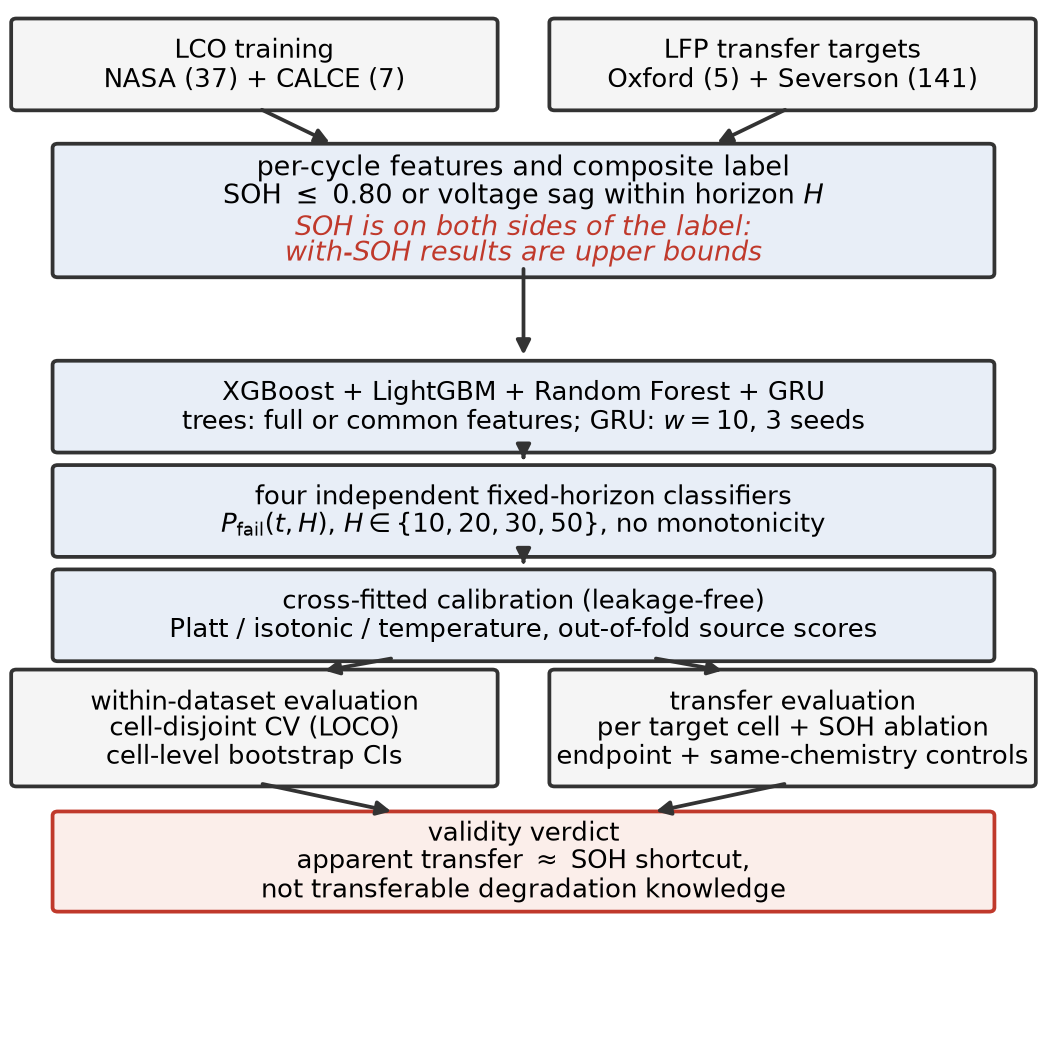
\includegraphics[width=\columnwidth]{figs/fig_framework.png}
\caption{Overview of the proposed multi-horizon failure-risk framework.}
\label{fig:framework}
\end{figure}

\subsection{Datasets and Feature Representation}
Four public datasets spanning two battery chemistries are used
(Table~\ref{tab:datasets}). The NASA PCoE~\cite{saha2007} and CALCE
CX2~\cite{calce2023} datasets are used for training, while the Oxford
Battery Degradation Dataset~\cite{birkl2017} and MIT--Stanford
Severson~\cite{severson2019} datasets serve as cross-chemistry transfer
targets. A battery is labeled as failed when SOH falls below 0.80 or
the average voltage sag drops below 94\% of the first ten-cycle
baseline.

\begin{table}[!t]
\caption{Summary of the Four Battery Datasets}
\label{tab:datasets}
\centering
\small
\begin{tabular}{|l|l|l|l|l|}
\hline
Dataset & Cells & Chem. & Cycles/Cell & Role\\
\hline
NASA 18650~\cite{saha2007} & 37 & LCO & 1--445 & Training\\
CALCE CX2~\cite{calce2023} & 7 & LCO & 775--1{,}961 & Training\\
Oxford LFP~\cite{birkl2017} & 5 & LFP & 46--78 & Transfer\\
Severson~\cite{severson2019} & 141 & LFP & 101--2{,}237 & Transfer\\
\hline
\end{tabular}
\end{table}

Two properties of these datasets matter for interpretation. First, the
Oxford release logs discharge summaries at roughly 100-cycle intervals,
so after preprocessing only 46--78 usable cycles per cell remain and
every horizon is shorter than the sampling interval; Oxford failure
labels are identical across all four horizons, and Oxford scores measure
pooled failure detection rather than horizon-resolved prediction
(per-cell statistics effectively cover four of its five cells). Second, because
chemistry, laboratory, cell manufacturer, cycling protocol, and logging
resolution all change simultaneously between any source and target, the
shift evaluated here is cross-\emph{dataset} as well as
cross-chemistry; ``cross-chemistry'' is used as shorthand and
Section~II-E describes the controls that separate the two.

The feature vector consists of standard battery management system (BMS)
measurements requiring no additional sensors,
\begin{equation}
x_t = \{\mathrm{SOH}_t, \bar{V}_t, I_t, T_t, \mathrm{dur}_t, t\},
\label{eq:features}
\end{equation}
used directly by the tree ensembles, while the GRU processes a rolling
window of $w=10$ cycles,
\begin{equation}
X_t^{(w)} = \left[x_{t-w+1},\, \ldots,\, x_t\right] \in \mathbb{R}^{w \times d}.
\label{eq:window}
\end{equation} In the CALCE dataset, average temperature and
duration are completely missing and are zero-imputed for the tree
models; this is harmless within a single dataset but a constant-zero
column can act as a dataset identifier in pooled training, which
Section~III-C controls for with a common-feature variant. The GRU
excludes those two features and uses only cycle, average voltage,
minimum voltage, and SOH during transfer; the tree ensembles are
additionally evaluated on this identical common feature set, so that
architecture and feature availability are not confounded when
comparing models under shift.

\subsection{Operational Reliability Formulation}
Rather than estimate SOH or remaining useful life directly, we predict
failure probability within a fixed operating horizon,
\begin{equation}
Y_{t,H} =
\begin{cases}
1, & \text{if failure occurs within } (t, t+H]\\
0, & \text{otherwise}
\end{cases}
\label{eq:label}
\end{equation}
with conditional failure probability
\begin{equation}
P_{\mathrm{fail}}(t, H) = P\!\left(T_f \le t + H \mid T_f > t,\; x_t\right),
\label{eq:prob}
\end{equation}
where $T_f$ is the failure cycle. This framing treats battery
prognostics as a discrete-time survival problem, aligned with how a BMS
would use the output operationally. Two honesty notes are essential.
First, (5) is a fixed-horizon \emph{cumulative failure-risk} target:
each horizon is an independent binary classifier, no cycle-level hazard
or survival product is estimated, and no monotonicity constraint
$P_{10}\le P_{20}\le P_{30}\le P_{50}$ is enforced (violations reach
up to 46\% of within-dataset rows), which is why we say
\emph{failure-risk classification} rather than hazard modeling.
Second, the label is \emph{partially defined by SOH itself} and SOH is
also an input feature (Eq.~\ref{eq:features}); with-SOH results are
upper bounds that include this label-proximity leakage, and
Section~III-E quantifies it directly.

\subsection{Models and Training}
We evaluate XGBoost (max\_depth 4, learning rate 0.05, subsample 0.8,
colsample 0.8, min\_child\_weight 5), LightGBM with matched
hyperparameters, Random Forest (300 trees, max\_depth 6), and a
single-layer GRU (8 hidden units, 10-cycle window, Adam at learning
rate 0.005, early stopping). Within-dataset evaluation uses 5-fold
cell-grouped cross-validation on NASA (37 cells) and
leave-one-cell-out on CALCE (7 cells): every cycle from a given cell
stays on one side of every split, models are retrained per horizon,
and the cell, not the cycle, is the experimental unit.

\subsection{Probability Calibration}
Raw predictions are calibrated with Platt scaling~\cite{platt1999},
\begin{equation}
P_{\mathrm{cal}} = \frac{1}{1 + \exp(A\,s + B)},
\label{eq:platt}
\end{equation}
which fits the logistic parameters $A$ and $B$ on out-of-fold scores
$s$, and isotonic regression~\cite{zadrozny2002},
\begin{equation}
P_{\mathrm{cal}} = g_{\mathrm{iso}}(s), \quad
g_{\mathrm{iso}} = \operatorname*{arg\,min}_{g\;\mathrm{non\mbox{-}decreasing}}
\textstyle\sum_i \bigl(y_i - g(s_i)\bigr)^2,
\label{eq:iso}
\end{equation}
a non-decreasing step fit, with temperature scaling ($P_{\mathrm{cal}}
= \sigma\!\left(\ln\tfrac{s}{1-s}\big/T\right)$) as a reference. The protocol is leakage-clean: calibrators are fitted only on
out-of-fold scores produced by an inner cell-disjoint split of the
training cells, and the untouched test cells are scored by a model
trained on all training cells. No calibrator is ever fitted on the
scores it is applied to, which removes the optimistic bias of in-sample
fitting (an earlier version of this study fitted calibrators directly
on training-fold predictions; the absolute calibration numbers here are
accordingly more conservative). Calibration quality
is assessed by the Brier score, expected calibration error (ECE, ten
equal-width bins), and the slope of a logistic recalibration of the
predicted probabilities (slope 1 indicates perfect probabilistic
calibration).

\subsection{Transfer Protocol and Statistical Testing}
Models are trained on NASA, CALCE, or their combination and evaluated
per cell on Oxford and Severson, with pooled results accompanied by
cell-level bootstrap 95\% confidence intervals (resampling cells, not
cycles). We consider two feature settings, the full feature set and
SOH removed, to test whether cross-chemistry performance reflects
transferable degradation or mainly depends on SOH, and additionally a
distance-to-threshold baseline that scores each cycle by the unfitted
rule $0.80-\mathrm{SOH}$, which is the correct first baseline if the
health state itself is what transfers. Significance is assessed with
the DeLong test~\cite{delong1988} as secondary evidence only: the test
treats every cycle-level prediction as independent, so within-cell
correlation inflates its $p$-values (pseudoreplication), and we read it
as a directional consistency check, never as a precise significance
statement.

\section{Results and Discussion}

\subsection{Within-Dataset Reliability}
Table~\ref{tab:within} shows fold-mean Platt-calibrated AUC per
horizon. Every one of the 32 model--horizon--dataset combinations
reaches a fold-mean AUC of at least 0.85 under the clean protocol
(Fig.~\ref{fig:horizons}); the GRU shows the largest fold-to-fold
variance while the tree ensembles remain stable, and Brier scores stay
low. Platt calibration preserves these rankings at comparable
calibration error (Table~\ref{tab:calibration}).

\begin{table}[!t]
\caption{Within-Dataset Platt-Calibrated AUC and Brier Score}
\label{tab:within}
\centering
\small
\setlength{\tabcolsep}{3.4pt}
\begin{tabular}{|l|l|c|c|c|c|c|c|}
\hline
Model & Dataset & H=10 & H=20 & H=30 & H=50 & Mean & Brier\\
\hline
XGBoost & NASA & 0.903 & 0.899 & 0.910 & 0.918 & 0.907 & 0.182 \\
XGBoost & CALCE & 0.965 & 0.967 & 0.967 & 0.943 & 0.961 & 0.075 \\
LightGBM & NASA & 0.912 & 0.909 & 0.892 & 0.901 & 0.903 & 0.206 \\
LightGBM & CALCE & 0.967 & 0.968 & 0.943 & 0.942 & 0.955 & 0.075 \\
Random Forest & NASA & 0.911 & 0.901 & 0.912 & 0.927 & 0.913 & 0.201 \\
Random Forest & CALCE & 0.934 & 0.933 & 0.917 & 0.903 & 0.922 & 0.070 \\
GRU & NASA & 0.872 & 0.893 & 0.884 & 0.856 & 0.876 & 0.307 \\
GRU & CALCE & 0.952 & 0.959 & 0.935 & 0.921 & 0.942 & 0.130 \\
\hline

\end{tabular}
\end{table}

\begin{figure}[!t]
\centering
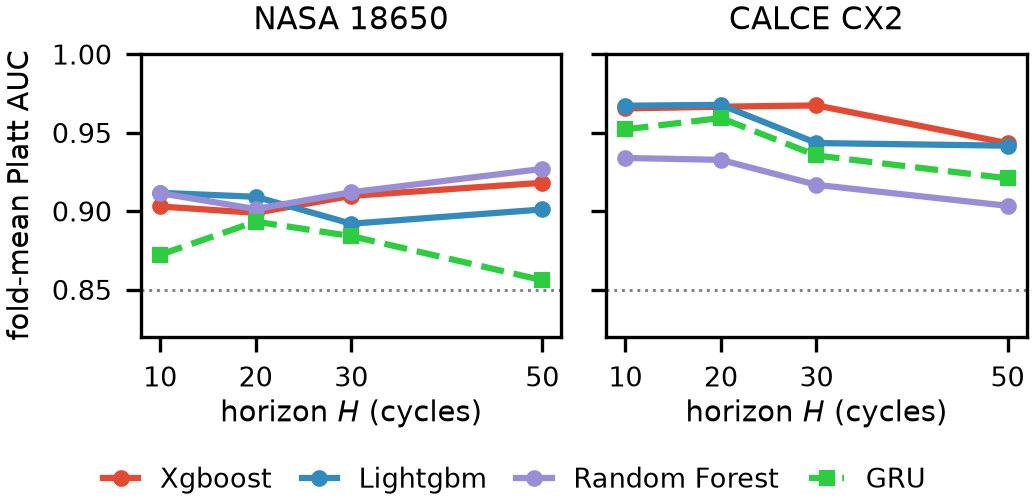
\includegraphics[width=\columnwidth]{figs/fig_within_horizons.png}
\caption{Within-dataset fold-mean Platt AUC across horizons.}
\label{fig:horizons}
\end{figure}

\begin{table}[!t]
\caption{Calibration Method Comparison (Mean Across Tree Models)}
\label{tab:calibration}
\centering
\small
\begin{tabular}{|l|l|c|c|c|c|}
\hline
Dataset & Method & AUC & Brier & ECE & Slope\\
\hline
NASA & Isotonic & 0.854 & 0.207 & 0.151 & 0.48 \\
NASA & Platt & 0.908 & 0.196 & 0.136 & 0.90 \\
NASA & Temperature & 0.908 & 0.178 & 0.107 & 1.22 \\
CALCE & Isotonic & 0.915 & 0.067 & 0.049 & 0.41 \\
CALCE & Platt & 0.946 & 0.073 & 0.029 & 0.01 \\
CALCE & Temperature & 0.945 & 0.080 & 0.067 & 0.53 \\
\bottomrule

\end{tabular}
\end{table}

\subsection{Calibration: Platt Preserves Discrimination Best}
Table~\ref{tab:calibration} compares the three calibrators. A fitted
calibrator is a monotone re-mapping, so per-fold ranking is preserved
up to the ties it introduces and fold-mean AUC differences are small;
but isotonic's tied step groups cost precision--recall dearly, and
Platt's fitted slope on CALCE is only 0.01: under
leave-one-cell-out the out-of-fold sigmoid washes confidence toward
the base rate while preserving ranking. We therefore read the
comparison as: Platt \emph{preserves discrimination best while
achieving calibration error comparable to or better than isotonic},
a materially weaker and more defensible claim than ``Platt is the
better calibrator'', and raw scores remain the safest ranking signal
whenever the operating context is uncertain
(Fig.~\ref{fig:reliability}).

\begin{figure}[!t]
\centering

\includegraphics[width=\columnwidth]{figs/fig_reliability_v2.png}
\caption{Reliability diagrams under the cross-fitted protocol. (a)
Within CALCE. (b) ALL-LCO$\to$Severson without SOH.}
\label{fig:reliability}
\end{figure}

\subsection{Cross-Dataset Transfer and the SOH Shortcut}
Table~\ref{tab:transfer} compares transfer at $H{=}20$ with and
without SOH as a feature; transfer is reported in raw AUC because
calibration parameters are dataset-specific. With SOH included, the
tree ensembles reach pooled AUC between 0.85 and 1.00. Removing SOH
collapses every tree model: on NASA+CALCE$\to$Oxford, XGBoost falls
from 0.917 to 0.429, no no-SOH configuration exceeds 0.58 on Oxford or
0.77 on Severson, and several fall below chance: the remaining
sensors rank the target distribution backwards. The GRU is highly
unstable across training seeds under shift (per-cell AUC from 0.21 to
1.00 at fixed settings) and offers no transfer advantage even though it
sees the same common feature set as the trees in the matched
comparison.

\begin{table}[!t]
\caption{Cross-Dataset Transfer at $H{=}20$ With and Without SOH}
\label{tab:transfer}
\centering
\resizebox{\columnwidth}{!}{%
\begin{tabular}{|l|l|c|c|}
\hline
Training & Model & Oxford (w/$-$SOH) & Severson (w/$-$SOH)\\
\hline
NASA & XGBoost & 0.957 & 0.518 & 0.871 & 0.595 \\ \hline
NASA & LightGBM & 1.000 & 0.533 & 0.849 & 0.527 \\ \hline
NASA & Random Forest & 1.000 & 0.521 & 0.861 & 0.674 \\ \hline
NASA & GRU & 0.143 & 0.152 & 0.832 & 0.766 \\ \hline
CALCE & XGBoost & 0.850 & 0.416 & 0.850 & 0.682 \\ \hline
CALCE & LightGBM & 0.889 & 0.462 & 0.863 & 0.643 \\ \hline
CALCE & Random Forest & 0.850 & 0.501 & 0.902 & 0.665 \\ \hline
CALCE & GRU & 0.120 & 0.100 & 0.777 & 0.524 \\ \hline
NASA+CALCE & XGBoost & 0.917 & 0.429 & 0.896 & 0.750 \\ \hline
NASA+CALCE & LightGBM & 0.971 & 0.332 & 0.882 & 0.718 \\ \hline
NASA+CALCE & Random Forest & 0.989 & 0.581 & 0.889 & 0.746 \\ \hline
NASA+CALCE & GRU & 0.053 & 0.015 & 0.799 & 0.748 \\ \hline

\end{tabular}}
\end{table}

\begin{figure}[!t]
\centering

\includegraphics[width=\columnwidth]{figs/fig_collapse_map.png}
\caption{Transferability collapse map at $H{=}20$.}
\label{fig:collapse}
\end{figure}

A first control is the distance-to-threshold rule
$0.80-\mathrm{SOH}$, which involves no fitting at all: it transfers to
Severson at pooled AUC 0.912 (95\% CI [0.84, 1.00]) for the ALL-LCO
source, within the confidence range of the tuned ensembles, so most
of the apparent transfer is the SOH coordinate itself. The
remaining controls are the subject of the next subsection.

\subsection{Failure-Definition Ablation and Same-Chemistry Controls}
The ablation of Table~\ref{tab:faildef} relabels failure by a single
endpoint at a time (SOH $\le 0.80$ only, voltage sag only, or both),
and its signature is clean: with-SOH transfer \emph{tracks how much
SOH defines the label}. Under an SOH-only label (the model is, in
effect, reading the label criterion) transfer to Severson saturates at
0.985; under the combined label it is 0.896; relabeling by voltage sag
alone, a criterion SOH takes no part in, cuts it to 0.723, a drop of
roughly a quarter. The residual with-SOH advantage under the voltage
label (0.723 versus 0.611 without SOH) is consistent with genuine but
weak health-state information: cells far below nominal capacity do fail
sooner under almost any definition.

\begin{table}[!t]
\caption{Failure-Definition Ablation at $H{=}20$ (Pooled Raw AUC)}
\label{tab:faildef}
\centering
\resizebox{\columnwidth}{!}{%
\begin{tabular}{|l|c|c|c|c|}
\hline
 & \multicolumn{2}{c|}{Oxford} & \multicolumn{2}{c|}{Severson}\\
\cline{2-3}\cline{4-5}
Label endpoint & w/ SOH & no SOH & w/ SOH & no SOH\\
\hline
Combined (SOH or sag) & 0.917 & 0.429 & 0.896 & 0.750 \\ \hline
SOH only & 0.995 & 0.464 & 0.985 & 0.759 \\ \hline
Voltage sag only & --- & --- & 0.723 & 0.611 \\ \hline

\end{tabular}}
\end{table}

\begin{table}[!t]
\caption{Same-Chemistry Controls at $H{=}20$}
\label{tab:samechem}
\centering
\small
\begin{tabular}{|l|c|c|}
\hline
Pair & w/ SOH & no SOH\\
\hline
NASA$\to$CALCE (LCO$\to$LCO) & 0.870 & 0.849 \\ \hline
CALCE$\to$NASA (LCO$\to$LCO) & 0.543 & 0.566 \\ \hline
Severson$\to$Oxford (LFP$\to$LFP) & 0.997 & 0.471 \\ \hline
Oxford$\to$Severson (LFP$\to$LFP) & 0.688 & 0.500 \\ \hline

\end{tabular}
\end{table}

If the collapse were a chemistry effect, transfer should survive when
chemistry is held constant; Table~\ref{tab:samechem} shows it does
not. Severson$\to$Oxford (both LFP) reproduces the full pattern of the
cross-chemistry shifts: 0.997 with SOH collapsing to 0.471 without,
an inverted 0.428 on the common feature set; NASA$\to$CALCE
(both LCO) behaves like the cross-chemistry pairs. Conversely,
CALCE$\to$NASA stays near chance even with SOH, showing that a small,
heterogeneous source limits transfer in both directions. The supported
conclusion is deliberately narrower than ``SOH is
chemistry-specific'': much of the observed cross-dataset,
cross-chemistry discrimination is attributable to SOH, partly because
SOH defines the failure criterion itself, and same-chemistry controls
attribute the collapse to dataset shift at least as much as to
chemistry.

\subsection{Multi-Horizon Analysis, Monotonicity, and a Discrete-Time Hazard Model}
Across the fixed-horizon classifiers, fold-mean AUC varies by less than
0.05 over $H \in \{10,20,30,50\}$ on both training datasets
(Fig.~\ref{fig:horizons}), with slightly larger variation at short
horizons due to class imbalance. Because the four horizons are
independent classifiers, however, cumulative risk coherence is not
guaranteed: the requirement $P_{10} \le P_{20} \le P_{30} \le P_{50}$
is violated in 32--45\% of within-dataset rows and up to 96\% of rows
on the transferred Severson target: for a hazard-style output, an
incoherent quantity to quote to an operator.

\begin{table}[!t]
\caption{Fixed-Horizon Versus Hazard Model AUC}
\label{tab:hazard}
\centering
\small
\setlength{\tabcolsep}{3.0pt}
\begin{tabular}{|l|c|c|c|c|}
\hline
 & \multicolumn{2}{c|}{$H{=}20$} & \multicolumn{2}{c|}{$H{=}50$}\\
\cline{2-3}\cline{4-5}
Setting & Fixed & Hazard & Fixed & Hazard\\
\hline
NASA & 0.899 & 0.935 & 0.918 & 0.927 \\
CALCE & 0.967 & 0.893 & 0.943 & 0.889 \\
NASA$\to$\textit{Oxford} & 0.957 & 0.971 \\
NASA$\to$\textit{Severson} & 0.871 & 0.884 \\
CALCE$\to$\textit{Oxford} & 0.850 & 0.466 \\
CALCE$\to$\textit{Severson} & 0.850 & 0.737 \\
NASA+CALCE$\to$\textit{Oxford} & 0.917 & 0.314 \\
NASA+CALCE$\to$\textit{Severson} & 0.896 & 0.866 \\
\hline

\end{tabular}
\end{table}

We therefore also fit an explicit discrete-time hazard model. For each
observed cycle $t$ and offset $\ell \in \{1,\ldots,L\}$ with $L=50$,
the hazard conditional on the features measured at $t$ (operational: no
future measurements) is
\begin{equation}
h_\ell(t) = P\bigl(T_f = t+\ell \mid T_f \ge t+\ell,\; x_t\bigr),
\label{eq:hazarddef}
\end{equation}
estimated by one pooled classifier on the offset-expanded at-risk
training rows $(x_t, \ell)$ with $\ell$ as an additional input
feature. Cumulative failure risk follows the survival product
\begin{equation}
R(t, H) = 1 - \prod_{\ell=1}^{H} \bigl(1 - \hat h_\ell(t)\bigr),
\label{eq:survival}
\end{equation}
which is monotone non-decreasing in $H$ by construction and yields all
four horizons from a single fit (Table~\ref{tab:hazard}). Within datasets the survival product matches
the fixed-horizon classifier at no cost. Under transfer it inherits the
same SOH dependence as every other model (formulating the output does
not exempt the inputs from dataset shift) and behaves
source-dependently (0.97 down to 0.31 pooled on Oxford), but it removes
the monotonicity incoherence entirely: its violation rate is zero by
construction.

\subsection{Operational Cost Analysis}
AUC treats all errors as equal; a BMS does not. We select the decision
threshold on source out-of-fold scores with a 10\% false-alarm budget
and apply it unchanged to the target (Table~\ref{tab:operational}).
On Severson with SOH, the transferred threshold misses 32\% of target
failures while holding false alarms to 4\%; without SOH the miss rate
more than doubles to 70\% with the full budget spent, and calibrated
scores differ only marginally: under shift the ranking is the asset
and the ranking is what collapsed. On Oxford, nearly every row is
positive under the coarse pooled labels, so no discriminating
operating point exists at all (Section~II-B).

\begin{table}[!t]
\caption{Operational Evaluation at $H{=}20$ (Target FNR\% / FPR\%)}
\label{tab:operational}
\centering
\resizebox{\columnwidth}{!}{%
\begin{tabular}{|l|l|c|c|c|}
\hline
Target & Features & raw & Platt & Isotonic\\
\hline
Oxford & with SOH & 0 / 93 & 0 / 93 & 0 / 93 \\ \hline
Oxford & no SOH & 0 / 92 & 0 / 92 & 0 / 92 \\ \hline
Severson & with SOH & 32 / 4 & 32 / 4 & 31 / 6 \\ \hline
Severson & no SOH & 70 / 10 & 70 / 10 & 67 / 12 \\ \hline

\end{tabular}}
\end{table}

\begin{table}[!t]
\caption{SOH Ablation at $H{=}20$ With Bootstrap CI and DeLong $p$-Value}
\label{tab:soh}
\centering
\resizebox{\columnwidth}{!}{%
\begin{tabular}{|l|l|c|c|c|l|}
\hline
Target & Model & w/ SOH & w/o & $\Delta$AUC [CI] & DeLong $p$\\
\hline
Oxford & XGBoost & 0.917 & 0.429 & +0.488 (5 cells) & $7.2e-51$ \\
Oxford & LightGBM & 0.971 & 0.332 & +0.639 (5 cells) & $2.6e-64$ \\
Oxford & Random Forest & 0.989 & 0.581 & +0.409 (5 cells) & $6.5e-36$ \\
Severson & XGBoost & 0.896 & 0.750 & +0.146 [0.10, 0.23] & $<10^{-300}$ \\
Severson & LightGBM & 0.882 & 0.718 & +0.164 [0.13, 0.23] & $<10^{-300}$ \\
Severson & Random Forest & 0.889 & 0.746 & +0.143 [0.11, 0.23] & $<10^{-300}$ \\
\hline

\end{tabular}}
\end{table}

Table~\ref{tab:soh} states the central comparison with the cell as the
experimental unit. On Severson the bootstrap interval on $\Delta$AUC
excludes zero by a wide margin for every model; on Oxford the
equivalent interval is uninformative (five cells, effectively four)
and we say so rather than lean on the astronomically small cycle-level
DeLong $p$-values, which are inflated by pseudoreplication. Within-dataset
model comparisons at $H{=}20$ are mostly not significant after honest
accounting (DeLong on pooled rows: XGBoost vs.\ LightGBM $1.4\times10^{-2}$
on NASA, $6.9\times10^{-28}$ on CALCE; XGBoost vs.\ Random Forest
$3.3\times10^{-1}$ and $8.5\times10^{-1}$), so no architecture
superiority is claimed.

\section{Conclusion}
This paper presented a multi-horizon failure-risk framework for
predicting lithium-ion battery failure across multiple datasets and
chemistries, and used it to run a validity analysis rather than only a
benchmark. Under cell-disjoint evaluation with leakage-free
cross-fitted calibration, within-dataset performance is uniformly
strong (fold-mean AUC $\ge 0.85$ in all 32 model--horizon--dataset
combinations). The cross-dataset results support a narrower and more
useful conclusion than apparent transfer success suggests: much of the
observed cross-dataset, cross-chemistry discrimination is attributable
to SOH, partly because SOH defines the failure criterion itself
(quantified by the failure-endpoint ablation), rather than to
degradation information in the remaining measured features, and
same-chemistry controls attribute the collapse to dataset shift at
least as much as to chemistry. Platt scaling preserves discrimination
best at comparable calibration error, though no source-fitted
calibrator repairs calibration on the shifted target.

Several limitations bound these claims: the fixed-horizon
classifiers have no enforced monotonicity across horizons; Oxford's
coarse 100-cycle sampling limits it to pooled-detection use; CALCE
contributes only seven cells; cross-chemistry evaluation covered LCO
and LFP only; and all datasets are laboratory-scale. Future work will
extend the framework to minimal-feature baselines as standard
practice, controlled same-laboratory cross-chemistry campaigns,
continuous time-to-failure modeling, and validation on large-scale
industrial datasets.

\section*{Acknowledgment}
The authors would like to acknowledge the use of writing-support and
language-enhancement tools, including OpenAI ChatGPT, Grammarly, and
QuillBot, during the preparation of this manuscript. These tools were
used to assist with grammar correction, readability improvement,
language refinement, and sentence restructuring. All technical
content, analysis, interpretations, and research contributions are
those of the authors.

\balance
\begin{thebibliography}{26}

\bibitem{berecibar2016} M. Berecibar, I. Gandiaga, I. Villarreal, N. Omar, J. Van Mierlo, and P. Van den Bossche, ``Critical review of state of health estimation methods of Li-ion batteries for real applications,'' \emph{Renewable and Sustainable Energy Reviews}, vol. 56, pp. 572--587, 2016, doi: 10.1016/j.rser.2015.11.042.

\bibitem{xu2024} G. Xu, J. Xu, and Y. Zhu, ``LSTM-based estimation of lithium-ion battery SOH using data characteristics and spatio-temporal attention,'' \emph{PLoS ONE}, vol. 19, no. 12, Art. no. e0312856, 2024, doi: 10.1371/journal.pone.0312856.

\bibitem{bairwa2025} B. Bairwa, K. Pareek, and V. K. Jadoun, ``Cycle based state of health estimation of lithium-ion cells using deep learning architectures,'' \emph{Scientific Reports}, vol. 15, Art. no. 37078, 2025, doi: 10.1038/s41598-025-20995-7.

\bibitem{tetik2026} T. Tetik, ``Feature engineering and explainable artificial intelligence for state of health estimation of lithium-ion batteries,'' \emph{Journal of Energy Storage}, vol. 144, Art. no. 119873, 2026, doi: 10.1016/j.est.2025.119873.

\bibitem{jin2021} S. Jin, X. Sui, X. Huang, S. Wang, R. Teodorescu, and D.-I. Stroe, ``Overview of machine learning methods for lithium-ion battery remaining useful lifetime prediction,'' \emph{Electronics}, vol. 10, no. 24, Art. no. 3126, 2021, doi: 10.3390/electronics10243126.

\bibitem{li2026} Y. Li, H. Shi, S. Wang, Q. Huang, C. Liu, S. Nie, X. Jia, and T. Luo, ``A comprehensive review of remaining useful life prediction methods for lithium-ion batteries: Models, trends, and engineering applications,'' \emph{Journal of Energy Chemistry}, vol. 112, pp. 384--414, 2026, doi: 10.1016/j.jechem.2025.08.056.

\bibitem{thelen2024} A. Thelen, X. Huan, N. Paulson, S. Onori, Z. Hu, and C. Hu, ``Probabilistic machine learning for battery health diagnostics and prognostics---review and perspectives,'' \emph{npj Materials Sustainability}, vol. 2, Art. no. 14, 2024, doi: 10.1038/s44296-024-00011-1.

\bibitem{li2026lightgbm} H. Li, ``Battery health prediction of new energy vehicles based on LightGBM,'' in \emph{Proc. Int. Workshop on Advances in Deep Learning for Image Analysis and Computer Vision (IWADIC 2025)}, 2026, pp. 80--89, doi: 10.2991/978-94-6239-648-7\_10.

\bibitem{wang2021} Z. Wang, Q. Ma, and Y. Guo, ``Remaining useful life prediction of lithium-ion batteries based on deep learning and soft sensing,'' \emph{Actuators}, vol. 10, no. 9, Art. no. 234, 2021, doi: 10.3390/act10090234.

\bibitem{rastegarpanah2024} A. Rastegarpanah, M. E. Asif, and R. Stolkin, ``Hybrid neural networks for enhanced predictions of remaining useful life in lithium-ion batteries,'' \emph{Batteries}, vol. 10, no. 3, Art. no. 106, 2024, doi: 10.3390/batteries10030106.

\bibitem{sun2025} L. Sun, X. Huang, J. Liu, J. Song, and S. Wu, ``Remaining useful life prediction of lithium batteries based on jump connection multi-scale CNN,'' \emph{Scientific Reports}, vol. 15, Art. no. 32873, 2025, doi: 10.1038/s41598-025-08619-6.

\bibitem{ibraheem2025} R. Ibraheem, T. I. Cannings, T. Sell, and G. dos Reis, ``Robust survival model for the prediction of Li-ion battery lifetime reliability and risk functions,'' \emph{Energy and AI}, vol. 19, Art. no. 100465, 2025, doi: 10.1016/j.egyai.2024.100465.

\bibitem{li2024} T. Li, Z. Zhou, A. Thelen, D. A. Howey, and C. Hu, ``Predicting battery lifetime under varying usage conditions from early aging data,'' \emph{Cell Reports Physical Science}, vol. 5, no. 4, Art. no. 101891, 2024, doi: 10.1016/j.xcrp.2024.101891.

\bibitem{yao2024} J. Yao, Q. Gao, T. Gao, B. Jiang, and K. M. Powell, ``A physics-guided machine learning approach to capacity fading mechanism detection and fading rate prediction using early cycle data,'' \emph{Batteries}, vol. 10, no. 8, Art. no. 283, 2024, doi: 10.3390/batteries10080283.

\bibitem{pang2026} H. Pang, X. Qu, K. Chen, X. Yan, A. F. Burke, and J. Zhao, ``A transferable deep learning framework for cross-chemistry and cross-scale state of health estimation in lithium-ion batteries,'' \emph{Energy}, vol. 354, Art. no. 141079, 2026, doi: 10.1016/j.energy.2026.141079.

\bibitem{platt1999} J. C. Platt, ``Probabilistic outputs for support vector machines and comparisons to regularized likelihood methods,'' in \emph{Advances in Large Margin Classifiers}, Cambridge, MA, USA: MIT Press, 1999, pp. 61--74.

\bibitem{zadrozny2002} B. Zadrozny and C. Elkan, ``Transforming classifier scores into accurate multiclass probability estimates,'' in \emph{Proc. 8th ACM SIGKDD Int. Conf. Knowledge Discovery and Data Mining}, Edmonton, AB, Canada, 2002, pp. 694--699.

\bibitem{goldstein2020} M. Goldstein, X. Han, A. Puli, and R. Ranganath, ``X-CAL: Explicit calibration for survival analysis,'' in \emph{Advances in Neural Information Processing Systems 33 (NeurIPS 2020)}, 2020, pp. 12759--12771.

\bibitem{lundberg2017} S. M. Lundberg and S.-I. Lee, ``A unified approach to interpreting model predictions,'' in \emph{Advances in Neural Information Processing Systems 30 (NeurIPS 2017)}, 2017, pp. 4768--4777.

\bibitem{dosreis2021} G. dos Reis, C. Strange, M. Yadav, and S. Li, ``Lithium-ion battery data and where to find it,'' \emph{Energy and AI}, vol. 5, Art. no. 100081, 2021, doi: 10.1016/j.egyai.2021.100081.

\bibitem{li2025} D. Li, J. Nan, A. F. Burke, and J. Zhao, ``Battery prognostics and health management: AI and big data,'' \emph{World Electric Vehicle Journal}, vol. 16, no. 1, p. 10, 2025, doi: 10.3390/wevj16010010.

\bibitem{delong1988} E. R. DeLong, D. M. DeLong, and D. L. Clarke-Pearson, ``Comparing the areas under two or more correlated receiver operating characteristic curves: A nonparametric approach,'' \emph{Biometrics}, vol. 44, no. 3, pp. 837--845, 1988.

\bibitem{severson2019} K. A. Severson, P. M. Attia, N. Jin, et al., ``Data-driven prediction of battery cycle life before capacity degradation,'' \emph{Nature Energy}, vol. 4, pp. 383--391, 2019, doi: 10.1038/s41560-019-0356-8.

\bibitem{saha2007} B. Saha and K. Goebel, ``Battery Data Set,'' NASA Ames Prognostics Data Repository, NASA Ames Research Center, Moffett Field, CA, USA, 2007.

\bibitem{calce2023} CALCE Battery Research Group, ``Battery aging datasets,'' Center for Advanced Life Cycle Engineering, Univ. of Maryland, College Park, MD, USA, 2023.

\bibitem{birkl2017} D. Howey and C. Birkl, ``Oxford Battery Degradation Dataset 1,'' Univ. of Oxford, Oxford, U.K., 2017.

\end{thebibliography}


\end{document}
